% small.tex
\documentclass{beamer}
\usetheme{Warsaw}

\usepackage[finnish]{babel}
\usepackage{lmodern}
\usepackage[utf8]{inputenc}
\usepackage[T1]{fontenc}
\usepackage{graphicx}

\title[Google Similarity Distance]{Google Samankaltaisuusetäisyys}
% \subtitle[Errors]{Estimation of numerical errors}
\author[T. Sand]{Timo Sand}
\institute[UH]{
  Tietojenkäsittelytieteen laitos\\
  Helsingin Yliopisto\\
  Helsinki\\[1ex]
}
\date[November 2013]{14. Marraskuu, 2013}

\begin{document}

\begin{frame}[plain]
  \titlepage
\end{frame}

\begin{frame}{Johdanto}
  \begin{itemize}
    \item Internet on miljoonien käyttäjien täyttämä tietokanta
    \item Melkein jokainen mahdollinen aihe on katettu
    \item Sisällöt keskimäärin huonolaatuisia
    \item Aiheitten matala-arvoisa approksimaatioita
  \end{itemize}

  \begin{itemize}
    \item GSD on yleinen menetelmä hyödyntää tätä huonolaatuista, ilmaista tietoa
    \item Maailman suurin semanttinen sahköinen tietokanta
    \item Hakukone palauttaa sivunumeroarvion mille tahansa hakukyselylle
  \end{itemize}

\end{frame}

\begin{frame}{Jäsentely}

\begin{itemize}
  \item Esimerkki
  \item Algoritmin perusta
  \item Samankaltaisuuden googlaus
  \item Sovellukset ja kokeilut
  \item Kertaus
\end{itemize}

\end{frame}

\begin{frame}{Esimerkki}
  \iffalse
horse:248 000 000
rider: 103 000 000
both: 72 600 000
  \fi
  \begin{itemize}
    \item Google haku sanoille "horse" ja "rider"
    \item Kirjataan sivujen lukumäärät, yksittäin ja yhdessä
    \item Maaliskuu 2007 $NGD('horse', 'rider') \approx 0.443$
    \item Marraskuu 2013 $NGD('horse', 'rider') \approx 0.233$
    \item Asteikko $0-1$
  \end{itemize}
\end{frame}

\begin{frame}{Algoritmin Perusta: Kolmogorov-kompleksisuus}
  Kolmogorov-kompleksisuus merkkijonosta $x$ on lyhimmän tietokoneohjelman pituus, joka tuottaa merkkijonon $x$.
   Jokaista olemassaolevaa pakkausalgoritmiä kohtaan meillä on $K(x) \leq$ pakatun $x$:n pituus.
\end{frame}

\begin{frame}{Normalisoitu informaatioetäisyys}
  \iffalse
  Lyhimmän tietokoneohjelman pituus, joka tuottaa merkkijonon x syötteellä y, sekä merkkijonon y syötteellä x; tätä pituutta kutsutan
  \fi
   \emph{Informaatioetäisyys}
    \[
    E(x, y) = K(x, y) - min\{K(x), K(y)\}
  \]

  \emph{Normalisoitu informaatioetäisyys}
    \[
      NID(x,y) =  \frac{K(x, y) - min\{K(x), K(y)\}}{max\{K(x), K(y)\}}
    \]
\end{frame}

\begin{frame}{Normalisoitu pakkausetäisyys}
\begin{itemize}
  \item NID ei ole laskettava, joten sitä ei voi tosielämässä käyttää.
  \item Pakkausalgoritmeillä ($C$) voi approksimoida Kolmogorov-kompleksisuuksia.
  \item $C(x)$ kuvastaa merkkijonon $x$ pakattua versiota
\end{itemize}
    \[
    NCD(x,y) =  \frac{C(xy) - min\{C(x), C(y)\}}{max\{C(x), C(y)\}}
    \]
\end{frame}

% \begin{frame}{Samankaltaisuuksien googlaus}
%   The number of Web pages currently indexed by Google is approaching $10^10$. Every common search term occurs in millions of Web pages. This number is so vast, and the number of Web authors generating Web pages is so enormous (and can be assumed to be a truly representative very large sample from humankind), that the probabilities of Google search terms, conceived as the frequencies of page counts returned by Google divided by the number of pages indexed by Google, approximate the actual relative frequencies of those search terms as actually used in society.
% \end{frame}

\begin{frame}{Google-jakauma}
  \begin{itemize}
    \item Yksittäisten hakujen joukko $S$
    \item Indeksöityjen internetsivujen joukko $\Omega$
    \item $M = |\Omega|$, joukon $\Omega$ mahtavuus
    \item Yksittäisiä hakuja $|S|$
    \item Yhdistettyjä hakuja $\binom{|S|}{2}$
    \item Määritellään $N = \sum_{\{x,y\}\subseteq S} |x \cap y|$
    \item $N \geq M$
  \end{itemize}
\end{frame}
\begin{frame}{Google samankaltaisuusetäisyys}
  \[
    NGD(x,y) = \frac{max\{\log f(x),\log f(y)\} - \log f(x,y)}{\log N - min\{\log f (x), \log f (y)\}}
  \]
    $f(x)$ ilmaisee sivujen lukumäärän, jokta sisältävät $x$:n, ja $f (x, y) $ ilmaisee sivujen lukumäärän, jotka sisältävät $x$:n ja $y$:n, Googlen mukaan.
\end{frame}
\begin{frame}{Sovellukset: Hierarkinen klusterointi}
  Hakusanoina: värit, numerot ja muutama konstikas sana
  \centering
  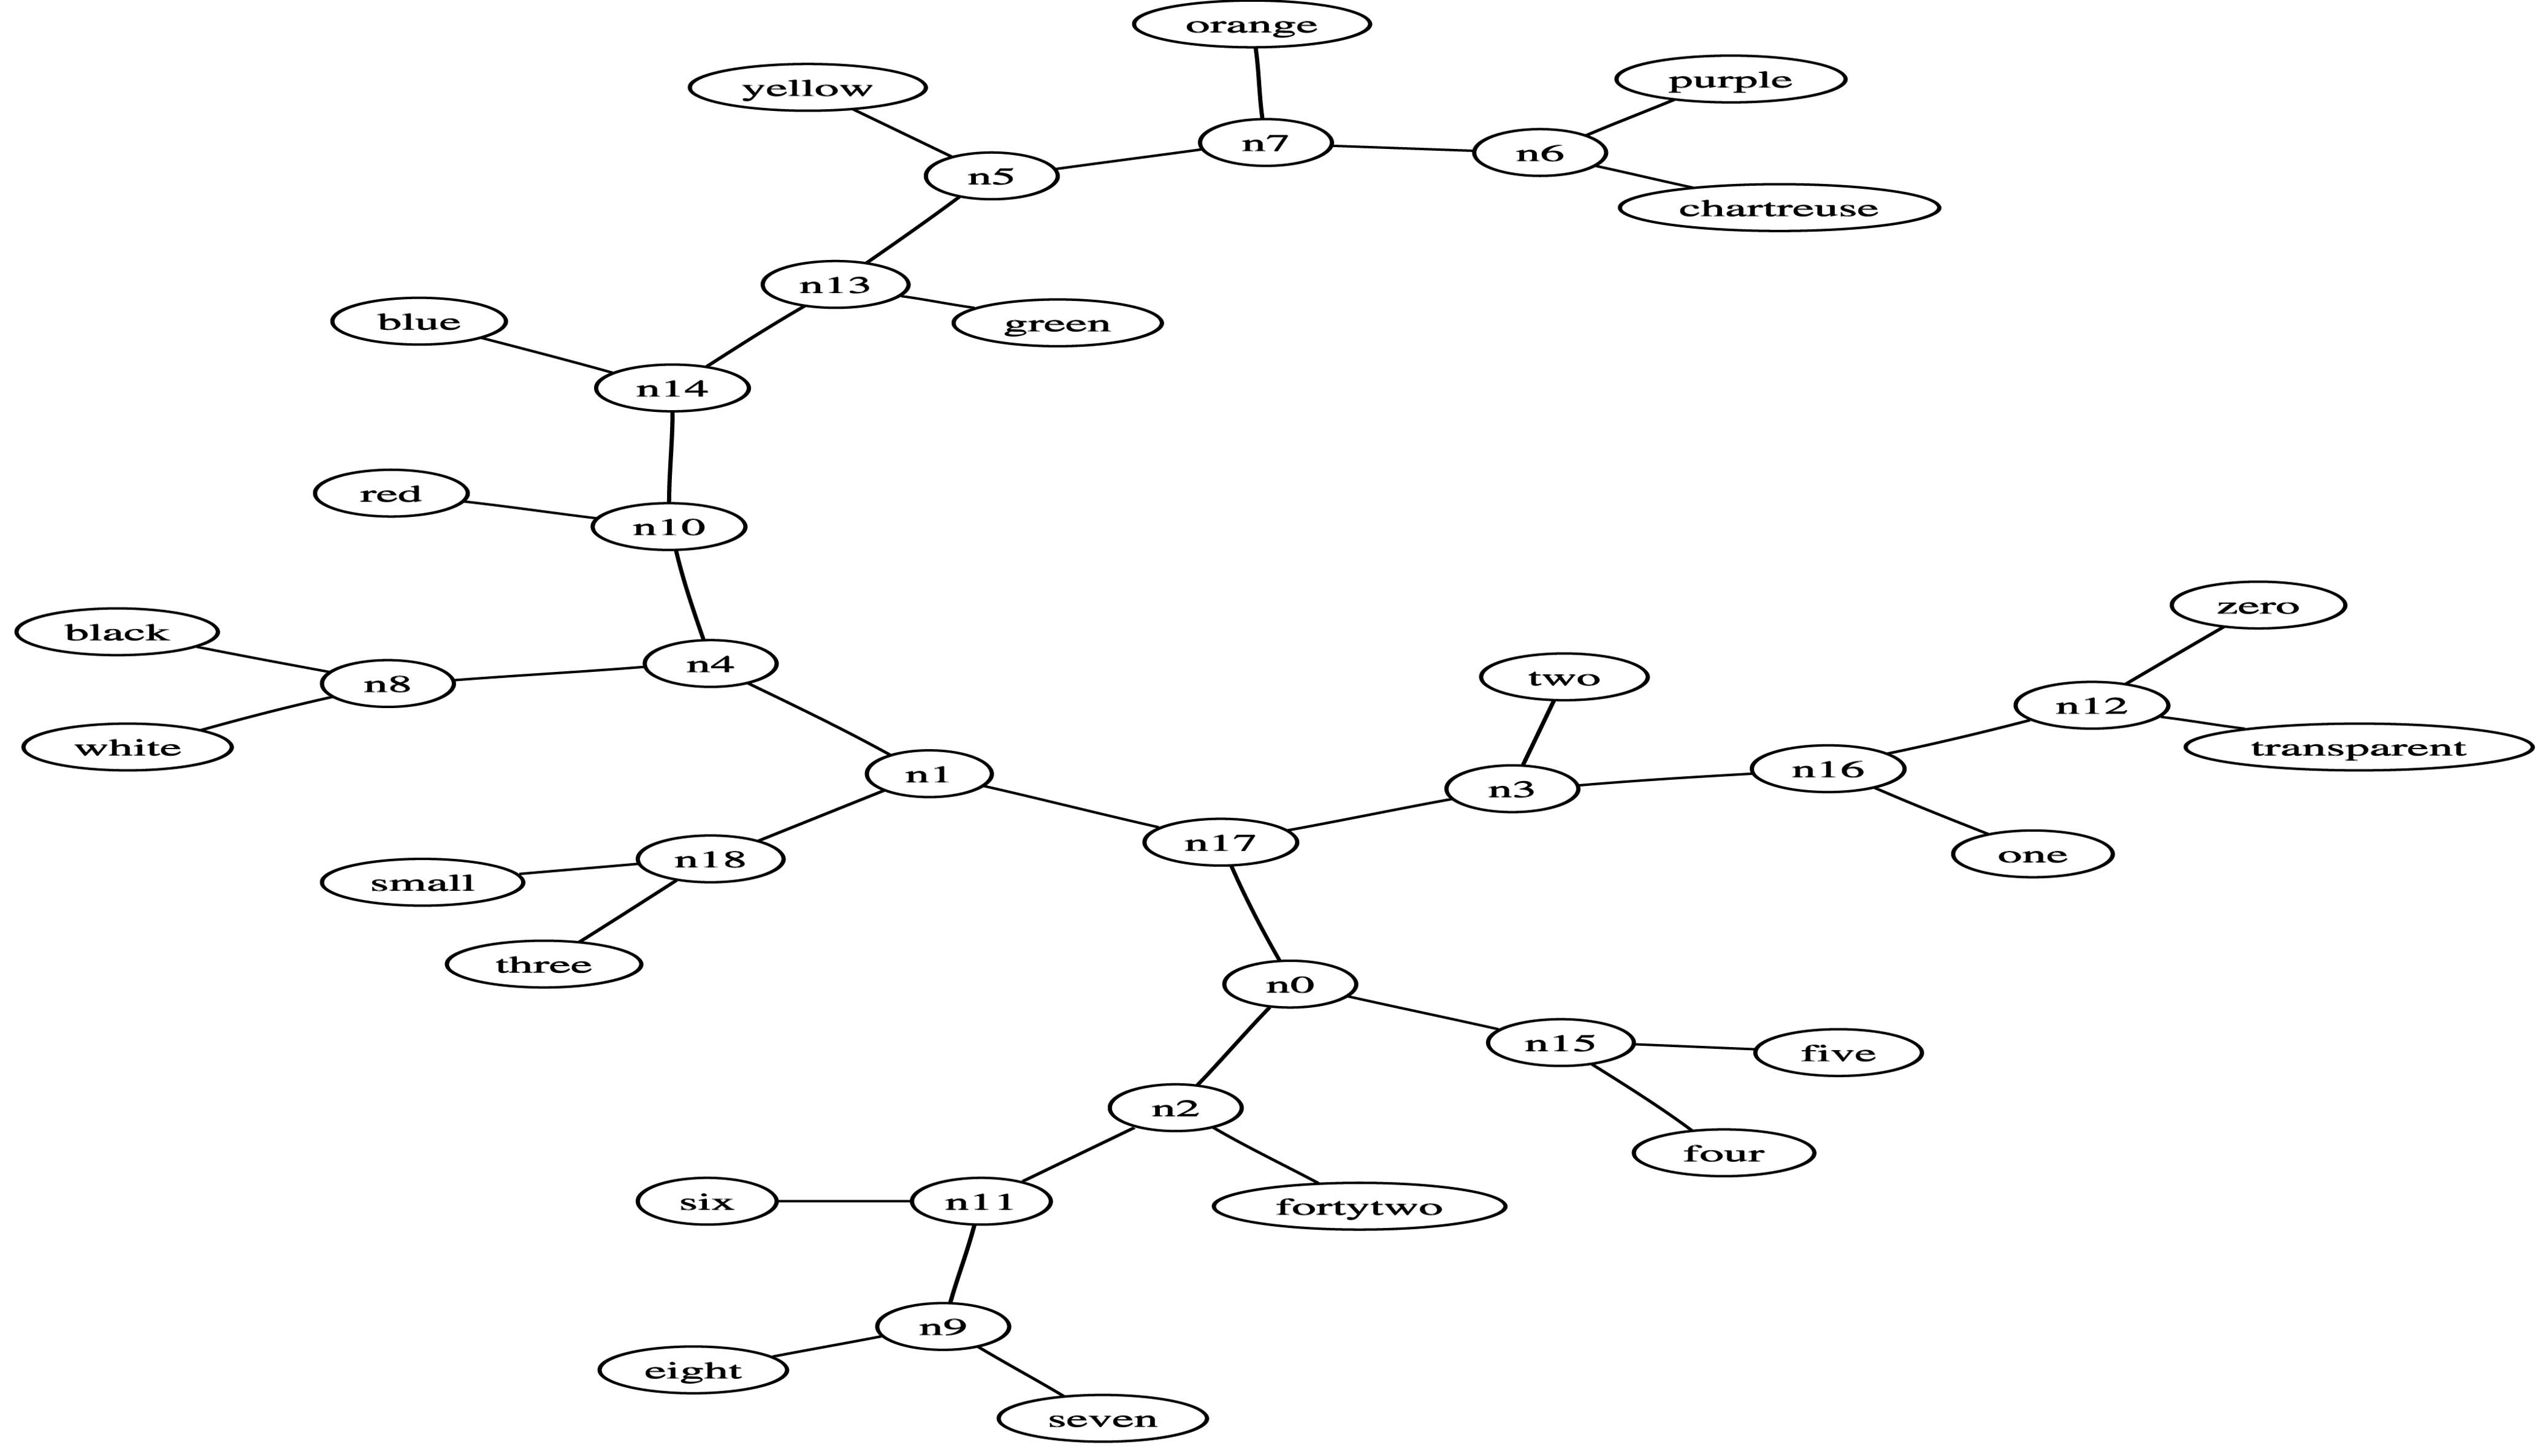
\includegraphics[width=8cm,keepaspectratio=true]{google-000}
\end{frame}

\begin{frame}{Sovellukset: Hollantilaisia maalareita}
  Hakusanoina 15 Steenin, Rembrandtin ja Bolin maalausta.
  \centering
  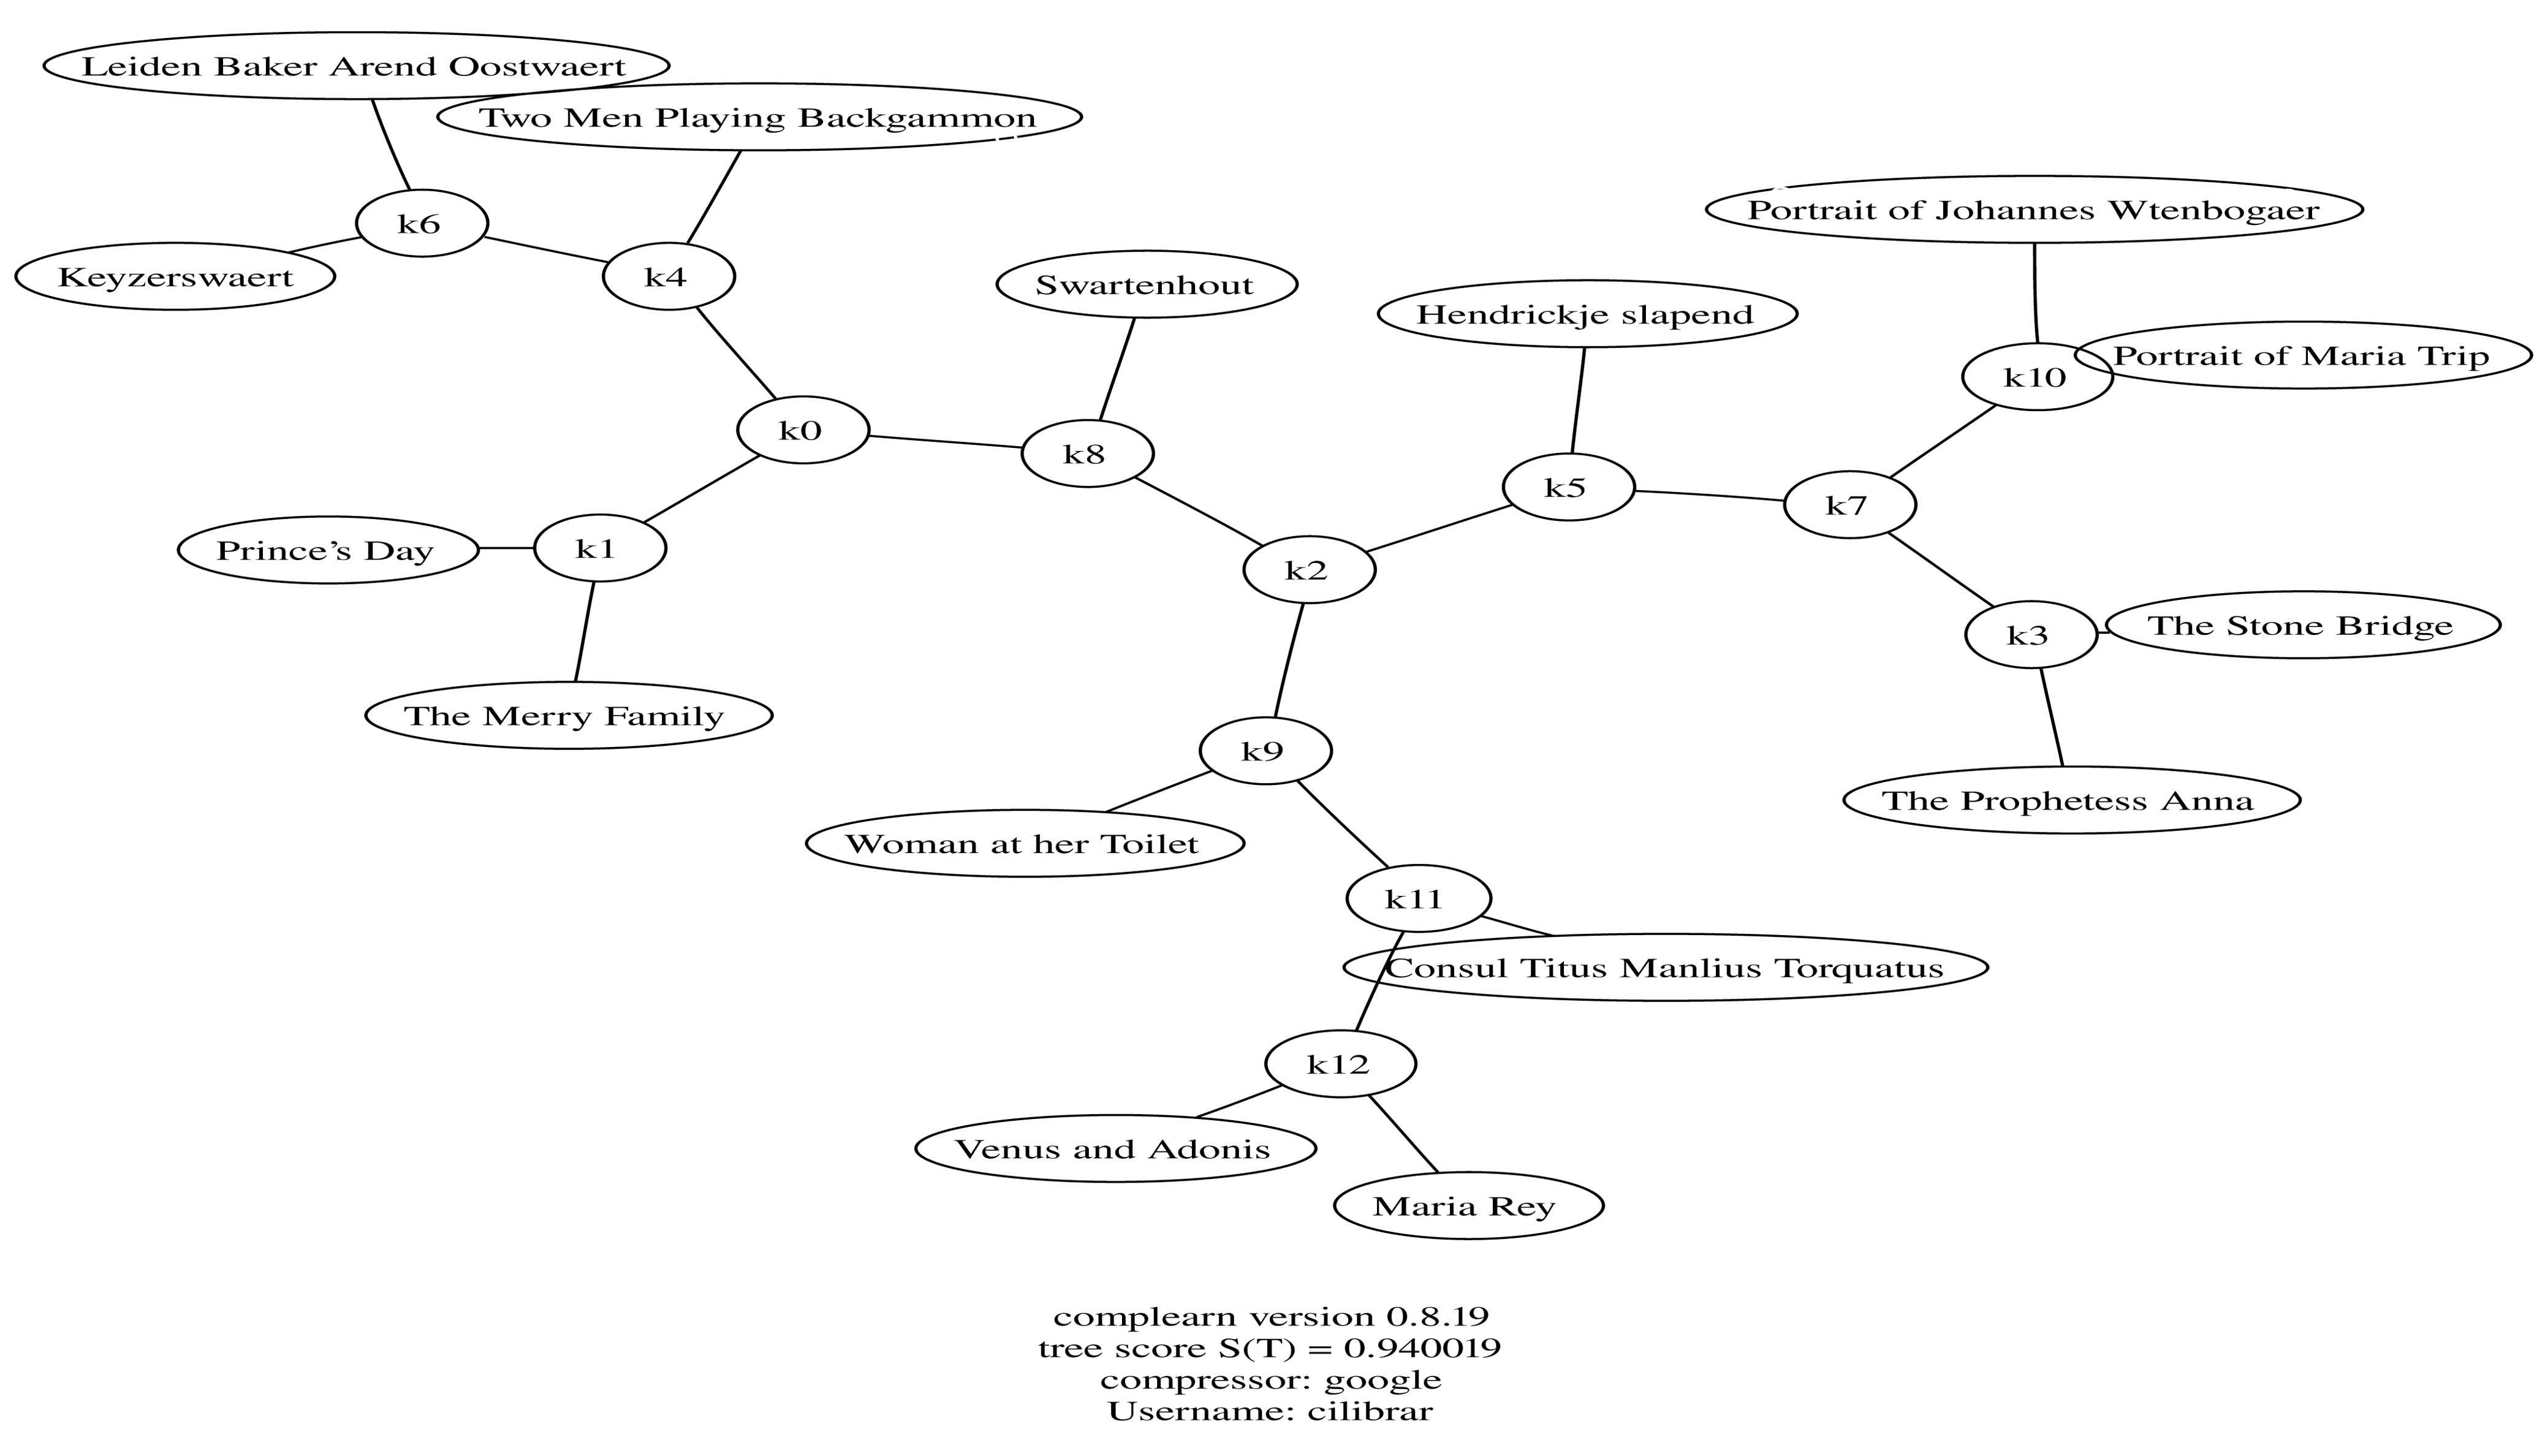
\includegraphics[width=8cm,keepaspectratio=true]{google-001}
\end{frame}

\begin{frame}{Sovellukset: Englantilaisia kirjailijoita}
  Hakusanoina Shakespearen, Oscar Wilden ja Jonathan Swiftin kirja
  \centering
  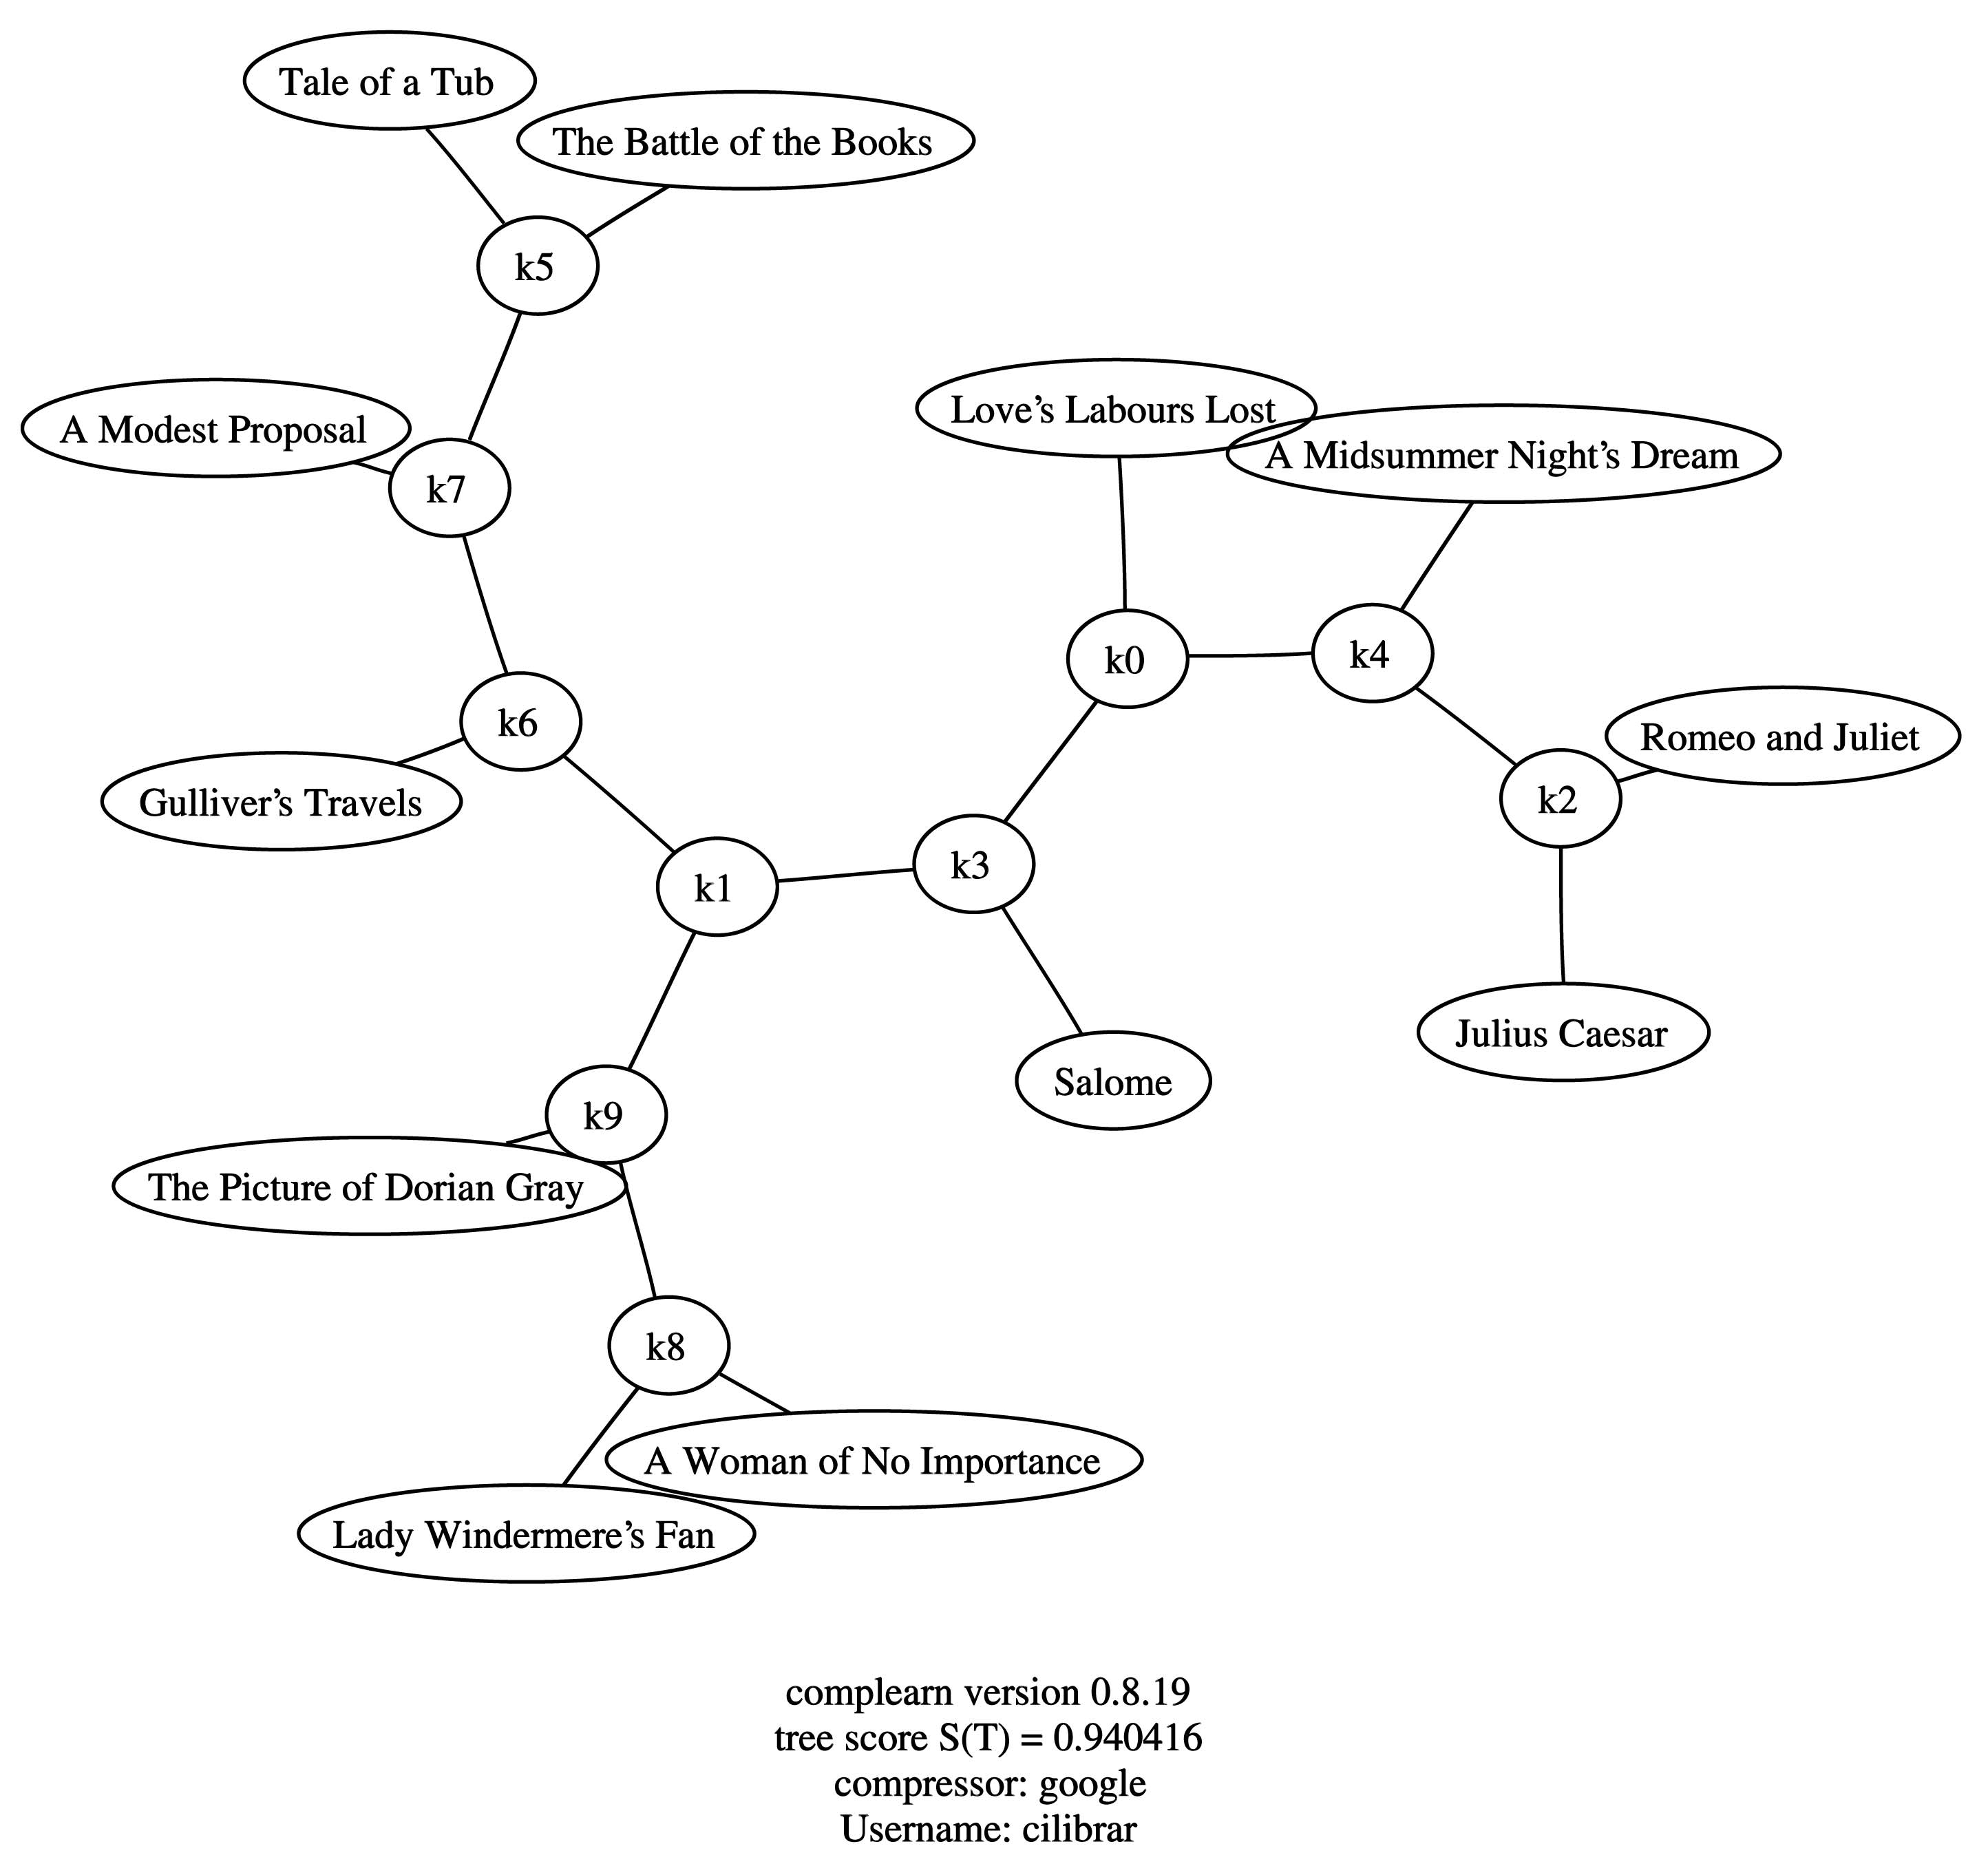
\includegraphics[width=8cm,keepaspectratio=true]{google-002}
\end{frame}

\begin{frame}{Kertaus}
  Kertaus
  \begin{itemize}
    \item NID
    \item NCD
    \item NGD
  \end{itemize}
\end{frame}

\begin{frame}
  \centering
  Kysymyksiä?
\end{frame}
\end{document}
